\section{System design}

\subsection{Physical layout}

The more detailed physical layout diagram shows the actual relations of the modules of the system to each other. There are several rapid prototyping technologies working together, all of them based on very high level languages.

The embedded system is running Angström Linux, which is a lightweight linux distribution. It enabled the use of Python and USB Hardware-extensions, a generic cheap USB Bluetooth Dongle and a webcam (The webcam is working, but it’s not supported yet on the software level).
Using Linux as the operating system of the embedded device has the additional advantage of manually controlling and updating the system through SSH.

The HLI and LLI are both implemented in Python. They communicate through function calls implemented via Cython. The actual Controller and Kalman Filter run natively, the .c/.h source code is compiled to .so files by the Cython compiler, which can be imported into the main python software as a static function library.

The source code files are generated by MATLAB Embedded Coder, based on the Simulink model of the control system. The resulting functions are more like objects, containing inner states and member functions, but only one instance can exist of the same controller object.

The GPIOs are controlled from Python as well, using system calls.

\begin{figure}[H]
	\centering
	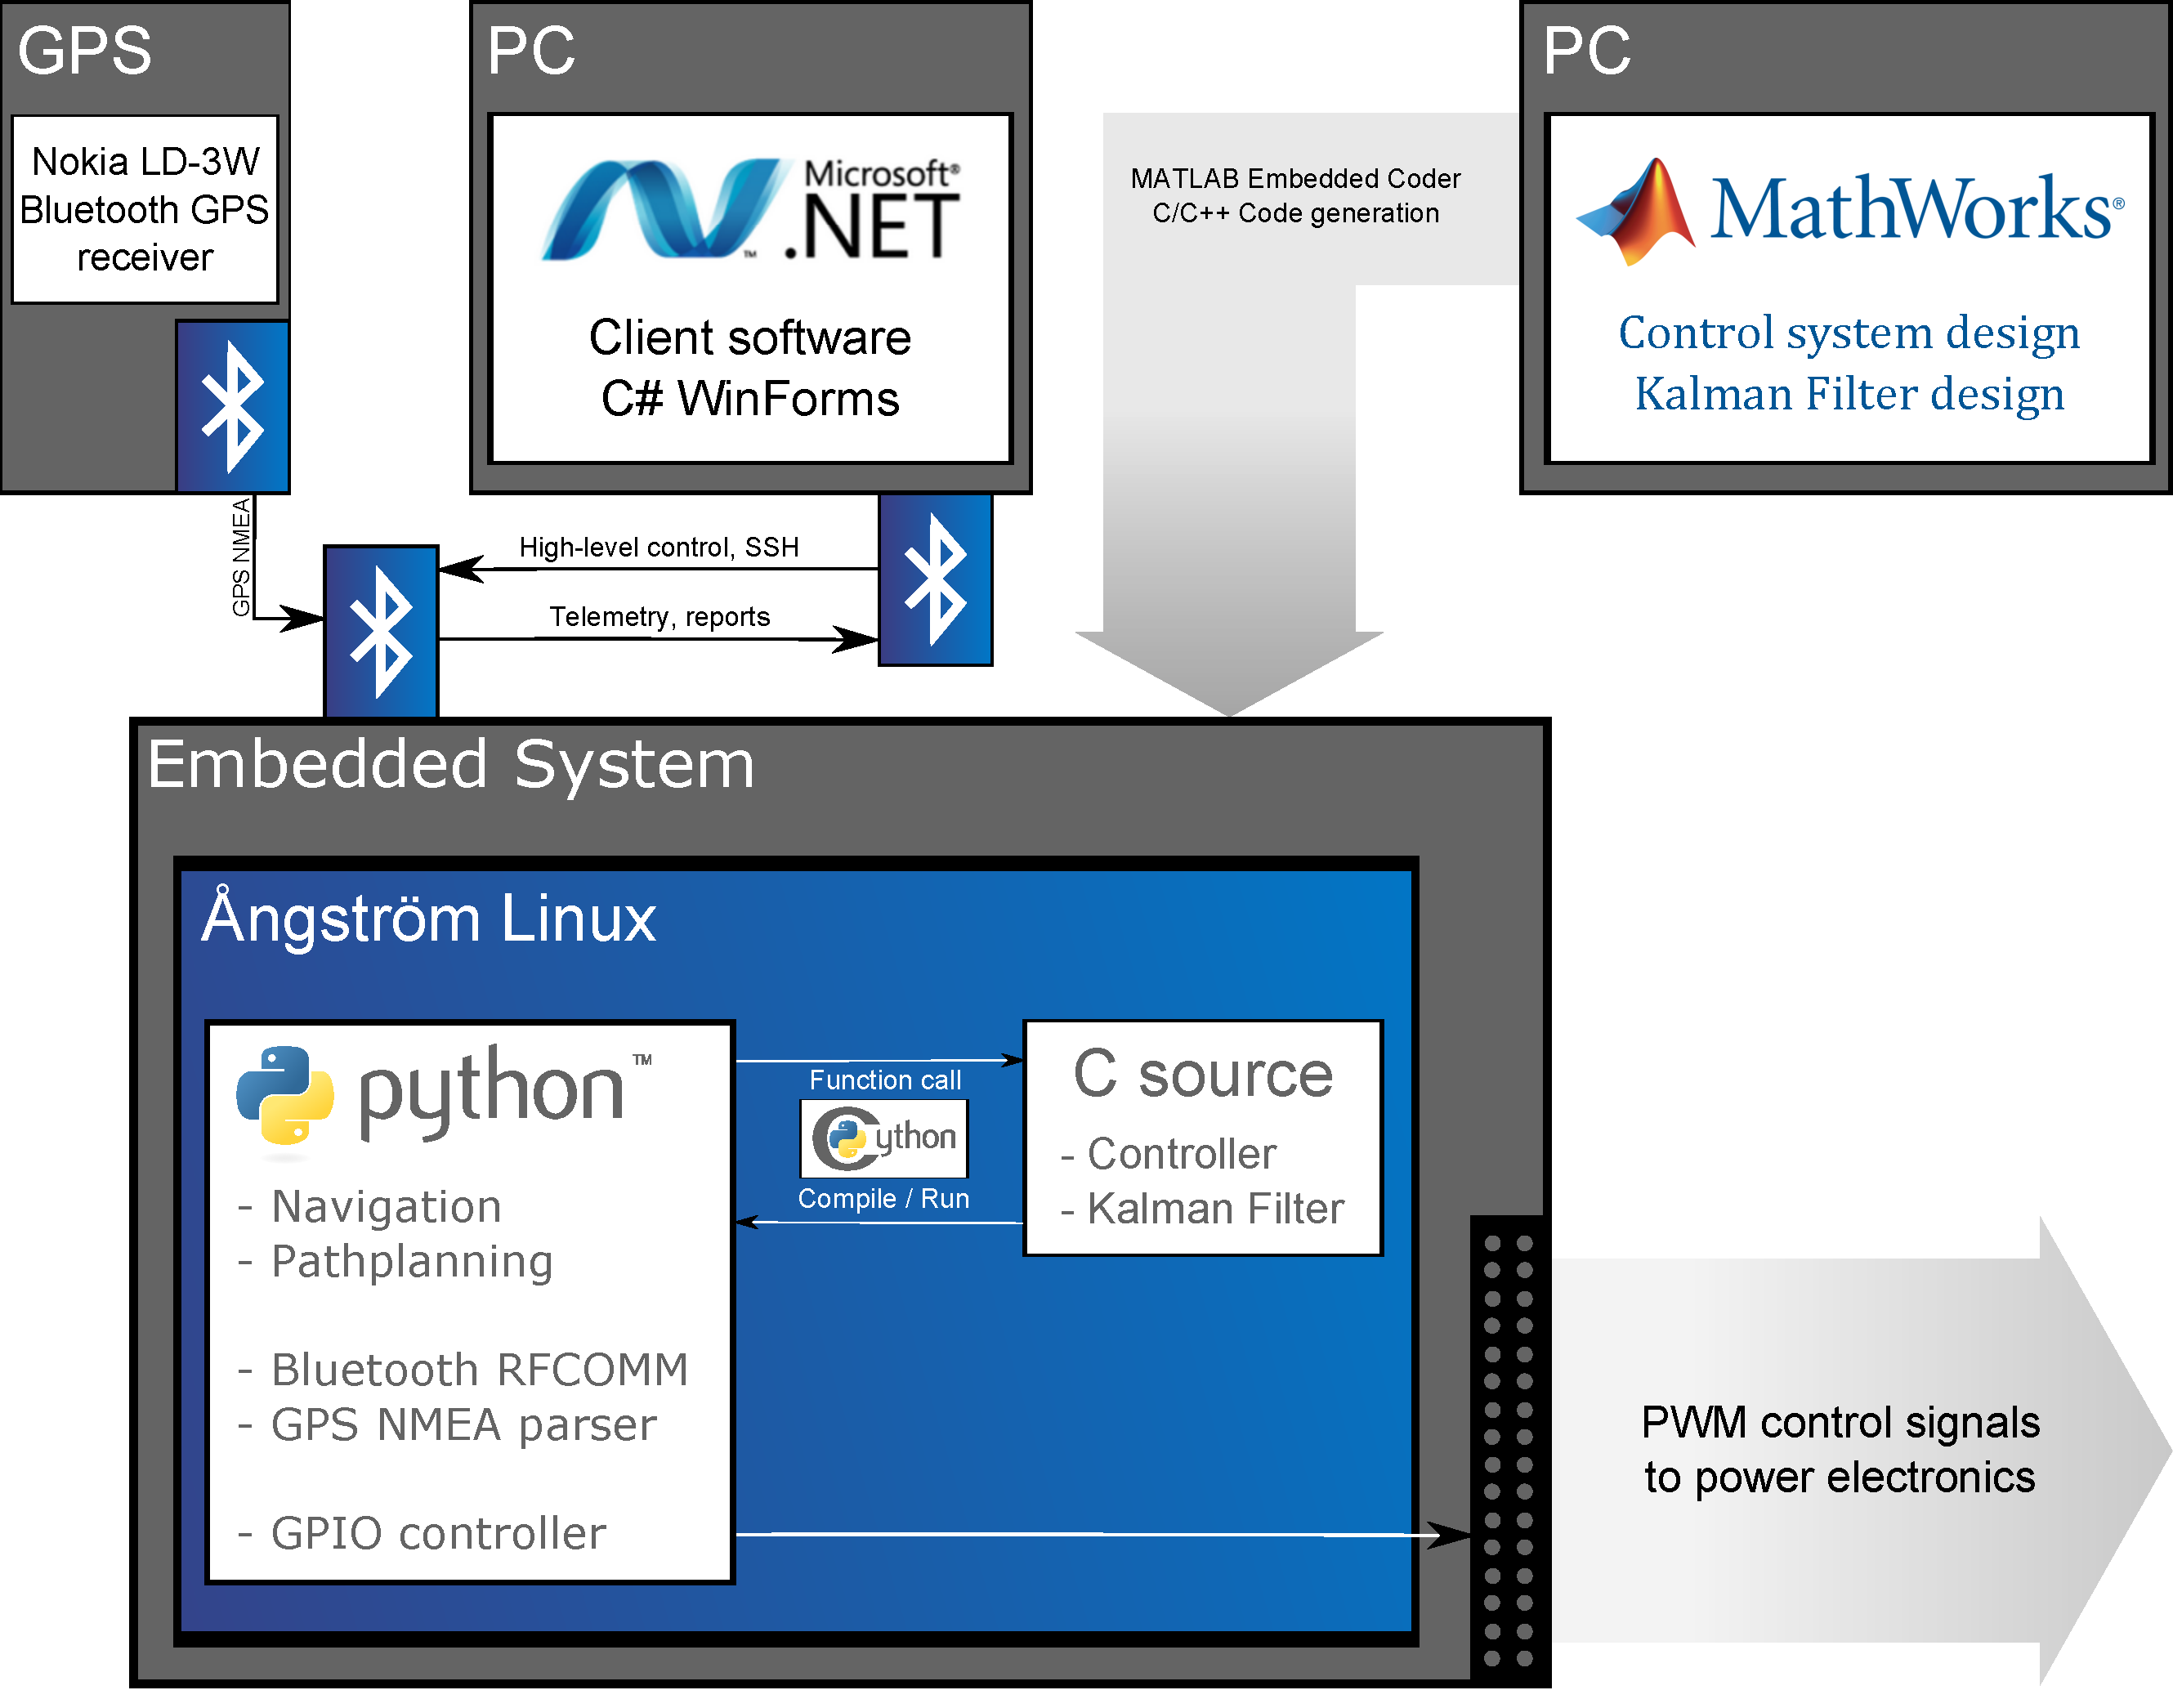
\includegraphics[width=1\textwidth]{img2/PhysicalLayout}
	\caption{The physical layout of the system}
	\label{fig:PhysicalLayout}
\end{figure}

The Embedded system has an USB Bluetooth hardware extension that communicates with the GPS receiver and the Client software.
It’s important to note, that the GPS receiver and the Embedded system are physically close to each other (relative to the scale of the ship), always within the range of the Bluetooth connection. Using wireless communication however enables the distant placement (relative to the scale of the circuit board) in order to ensure high GPS reception and a protected environment for the embedded system as well (e.g.: top of the mast and the belly of the boat).

\subsection{GPS Acquisition}

The localization procedure is implemented by a GPS (Global Positioning System) receiver, connected to the BBB via Bluetooth. The actual device is a Nokia LD-3W GPS device produced for Bluetooth-enabled smartphones without GPS connectivity. The receiver includes a battery with a relatively long life. Solar charging of the device is possible. [wrapfigure]
The Nokia LD-3W transforms the GPS signals to NMEA sentences that can be parsed to extract the current position, speed and much else. The NMEA 0183 is a standard marine serial electronics communication interface of the National Marine Electronics Association [\verb!www.nmea.org/content/nmea_standards/nmea_0183_v_410.asp! ].

The communication over the NMEA 0183 interface consists of NMEA sentences. There are many predefined sentence templates, but the Nokia LD-3W supports only some of them.

The beginning of each sentence is marked by a \$ character, immediately followed by the 5 character of the Sentence type that defines the interpretation. The data fields are submitted in a specific order, distinguished from each other by a comma character.

For the purpose of basic navigation, the processing of the GPRMA sentence is more than sufficient. A typical Sentence of this kind looks like the following:

(Graphic)
\$GPRMA, Data status, Latitude, N/S, Longitude, W/E, N/A, N/A, Speed, Course, Magnetic variation, Direction of variation(E/W), Checksum

\$ - Sentence start character
Data status - A = OK, B = Warning
Latitude - North / South position on the Globe. Lines of constant latitude run parallel to the equator.
Longitude - East / West position on the Globe. Lines of constant latitude run perpendicular to the equator.
Speed - Speed over ground, in knots
Course - Course over ground in degrees (90 -> East)
Magnetic variation - E/W angle correction required to apply to the compass at the current position to determine True North. Magnetic variation effect increases towards the poles.
Checksum - Can be checked for sentence errors.

Along the GPRMA, the GPGGA sentences provide useful informations about the position.

\$GPGGA, Time, Latitude, N/S, Longitude, E/W, Fix quality, Satellites, Precision, Altitude, Unit, Height above ellipsoid, Unit, DGPS last update, DGPS station ID, Checksum

Time - current time in HHMMSS
Fix quality - 0: no fix, 1: GPS fix, 2: DGPS fix
Satellites - Number of fixed satellites
Precision - Horizontal dilution of precision: sufficient under ~2.0[ref]
Altitude - Current altitude on a sphere
Height above ellipsoid - Height of Geoid above WGS84 ellipsoid: used for correction of Altitude

The GPS acquisition is implemented in Python by the Communication module of the HLI. The script uses linux-specific system calls to connect to the Bluetooth device and receive data, using the PyBluez module.

\subsection{Bluetooth connectivity}

\subsection{Sensors and effectors}